\documentclass[12pt]{article}
\usepackage[utf8x]{inputenc}
\usepackage[hebrew,english]{babel}
\usepackage{culmus}
\usepackage[yyyymmdd]{datetime}
\usepackage{amsmath,amssymb,amsthm}
\usepackage{graphicx}
\usepackage{textcomp}
\usepackage{mdframed}
\usepackage{lipsum}
\usepackage{cancel}
%general:
%Box and color definitions:
%--------------------------
\newenvironment{ColorBoxedminipage}
{\begin{minipage}} {\end{minipage}}
%{\begin{Sbox}\begin{minipage}}
%{\end{minipage}\end{Sbox}\fcolorbox{Blue}{White}{\TheSbox}}

%General definitions:
%-------------------
\newcommand{\etal}{{\em {et al.}}}
\newcommand{\B}[1]{\mathbf{#1}}
\newcommand{\df}{\triangleq}
\newcommand{\norm}[1]{\left\Vert#1\right\Vert}
\newcommand{\abs}[1]{\left\vert#1\right\vert}
\newcommand{\RE}{\operatorname{Re}}
\newcommand{\IM}{\operatorname{Im}}
\newcommand{\sgma}[3]{\sum\limits_{{#1}={#2}}^{#3}}
\newcommand{\Brace}[1]{\left\{{#1}\right\}} %Braces
\newcommand{\Brack}[1]{\left({#1}\right)} %Brackets
\newcommand{\sBrack}[1]{\left[{#1}\right]} %square Brackets

%\newcommand{\ip}[2]{{\langle{#1},{#2}\rangle}} %inner-product
\newcommand{\ipLW}[3]{{\langle{#1},{#2}\rangle}_{{#3}}} %weighted inner-product

\newcommand{\Tr}[1]{Tr\Brack{#1}}
\newcommand{\Mtr}[2] %short notation for 2x1 Matrix.
{\begin{bmatrix}
  #1 \\
  #2
\end{bmatrix}}
\newcommand{\cMtr}[2] %short notation for 2x1 Matrix with curves.
{\left(
\begin{array}{c}
    {#1} \\
    {#2} \\
\end{array}
\right)}
\newcommand{\Mtrs}[2] %short notation for 2x1 Matrix star (adjoint)
{\begin{bmatrix}
  #1 &
  #2
\end{bmatrix}}
\newcommand{\Mtrt}[3] %short notation for 3x1 Matrix.
{\begin{bmatrix}
  #1 \\
  #2 \\
  #3
\end{bmatrix}}

\newcommand{\Cases}[4]{
\left\{
\begin{tabular}{lcl}
    $#1$ & $=$ & $#2$\\
    $#3$     & $=$ & $#4$
\end{tabular}
\right. }

\newcommand{\und}{\underline} %How lazy can I get?
\newcommand{\ovr}{\overline}
\newcommand{\conj}[1]{{#1}^\ast} %Conjugation


\newcommand{\er}[1]{{(\ref{#1})}} %equation reference

\newtheorem{Lemma}{Lemma}{}
\newtheorem{Prop}{Proposition}{}
\newtheorem{theorem}{Theorem}{}


\newenvironment{alg}[5]
{
\begin{figure}[htbp]
\begin{center}
\fbox{
  \begin{ColorBoxedminipage}{13cm}
%    \leftline{\color{Black}\bf {#1}}
    {#4}
   \end{ColorBoxedminipage}
   }
\end{center}
  \bcaptionff{#1}{#2}{}{#3}
  \label{#5}
\end{figure}
}{}

%Just body, caption and label.
\newenvironment{algo}[3]
{
\begin{figure}[htbp]
\begin{center}
\fbox{
  \begin{ColorBoxedminipage}{7.5cm}
%    \leftline{\color{Black}\bf {#1}}
    {#1}
   \end{ColorBoxedminipage}
   }
\end{center}
  \caption{#2}
  \label{#3}
\end{figure}
}{}

\newenvironment{BOX}[1]
{
\begin{center}
\fbox{
  \begin{ColorBoxedminipage}{16cm}
%    \leftline{\color{Black}\bf {#1}}
    {#1}
   \end{ColorBoxedminipage}
   }
\end{center}
}{}

\newcommand\vecnot[1]{\boldsymbol{#1}}
\newcommand\optvecnot[1]{\vecnot{#1}_{opt}}

\usepackage{amsmath}
\DeclareMathOperator*{\argmax}{arg\,max}
\DeclareMathOperator*{\argmin}{arg\,min}

%Configuration-------------------------------------------------------------
\setlength{\parskip}{0.2cm}
\setlength{\parindent}{0cm}
\addto{\captionshebrew}{
    \renewcommand{\refname}{Bibliography}
    \renewcommand{\contentsname}{Table of Contents}
}
\newcommand{\printdate}[3]{{%
\day=#1\relax\month=#2\relax\year=#3\relax\today}}

\title{
\begin{otherlanguage}{hebrew}
התקדמות במחקר - יומן
\end{otherlanguage}
\\
Research progress - diary
}
\author{
\\Yehezkel Karo Itay
}
\begin{document}
\maketitle
\section*{Introduction}
Here one can see the latest progress, as for the past, in the ``spatial-IIR'' research. Weekly, on average, updates will be inserted here.
\section*{Pre-diary-creation progress}
We began by formulating the idea of Dr. Dvorkind of searching a suitable analogous spatial structure to the IIR filter.
A feedback based system was the main idea but the actual structure and math had to be developed.
We came across a certain PhD work \cite{van1988beamforming} of Fuxi Wen that tried to answer the same question but proposed different non-feedback based approaches which are examined in the research proposal.
His work was the only research that we found that actually tried to develop a spatial-only IIR beam-former.
As also mentioned in the research proposal, other papers \cite{Madanayake2008ABeamformer,Madanayake2009SystolicWDFs,Madanayake2008AFilters,Bruton2003Three-dimensionalBanks,Ward1986ABeamforming,Joshi2012SynthesisApplications} tried to create a spatio-temporal IIR beam-former but incorporating the time domain in the processing has its cones.
On 2017 Nov 11th, the final version of the research proposal was accepted.
\section{2017 Nov 15$^{th}$}
This week began with an initial simulation created by Dr. Dvorkind that applied a chebichev filter to the coefficients $ \vecnot{\alpha} $ and $ \vecnot{\beta} $.
The basic concept was proven but, when trying to implement in a simulated realized (coefficients quantization and partial knowledge of the $ \tau_{pd},\tau_{tx} $) environment, we noticed a very significant sensitivity of the systems response.
This led to a literature survey, trying to find a method for generating a low-sensitivity IIR filters in the context of coefficients quantization errors, assuming that those errors can also be interpreted as input modeling error in a high coefficients precision scenario.
Among the surveyed papers, we across an overview of IIR design methods \cite{ComplexIIRFilterDesign2011Zlatka}, which led us to find the first-order low-sensitivity IIR LS1b-structure \cite{I.P.Topalov1990LOW-SENSITIVITYCYCLES} and the second-order low-sensitivity IIR LS2-structure \cite{StoyanovNEWSECTIONS}.
The suggested method in \cite{ComplexIIRFilterDesign2011Zlatka} (page 15) was to ``Factor the transfer function to second-order (and possibly one first-order) terms and
design the corresponding LP/HP first and second-order filter sections. For each section apply
the Constantinides LP to LP spectral transformation 
$$ Z^{-1} \rightarrow \frac{z^{-1}-\beta}{1-\beta z^{-1}}=\mathcal{T}(Z) $$ 
This produces a composite multiplier coefficient $ \hat{\beta} $ that is a function of $ \beta $ and makes the BW variable''.
The near-future assignments will be:
\begin{itemize}
\item{
Verify that the MATLAB simulation is valid and no mistakes were made.
}
\item{
Update the simulation with the new transfer function factorization technique and validate that the overall response stays close to the original one and that the overall sensitivity is indeed minimized. 
}
\end{itemize}
\section{2017 Nov 23$^{rd}$}
This week's progress was mainly generating the presentation for the group meeting on Nov 27th (Monday).
\section{2017 Nov 27$^{th}$}
After presenting the research to Prof. Cohen's group, a few comments have been made.
\begin{itemize}
\item{
Missing motivation for the use of IIR over FIR. We were advised to create a slide that demonstrates a wanted spatial response and its resource usages in FIR vs. IIR.
}
\item{
Adding a slide of the intended quality factor which will be used to evaluate the system performance.
}
\item{
The presentation lacks a basic connection to a specific paper. Prof. Cohen would like to emphasize the fact that we are basing our research on an existing one.
}
\item{
It was brought to our attention that the transfer function actually depends also on the distance between the speaker and receiver. It could be interpreted as a feature, presenting a spatial 2D IIR filter which enhances a width-controlled radial slices in the medium.
}
\end{itemize}
\section{2017 Nov 29$^{th}$}
New papers were briefed:
\begin{itemize}
\item{
\textbf{``Spectral transformations for digital filters''} \cite{ConstantinidesTHEFilters}
\\
Deals with transforming low-pass filters to other kinds : Low-pass(other spec), high-pass, band-pass, band-stop. Features a table of the transformations.
}
\item{
\textbf{``Synthesis of variable IIR digital filters with complex coefficients''} \cite{Murakoshi1994SynthesisCoefficients}
\\
Not very relevant.
}
\item{
\textbf{``Design of limit-cycle-free digital biquad filters''} \cite{Nishihara1986DesignFilters}
\\
A method for removing limit-cycles from a given IIR.
\\
In \textbf{``NEW FIRST-AND SECOND-ORDER VERY LOW SENSITIVITY BANDPASS/BANDSTOP COMPLEX DIGITAL FILTER SECTIONS''}\cite{StoyanovNEWSECTIONS}, which is currently our main focus in the context of immunizing IIR filters, this paper is mentioned as the paper that suggests the most low-sensitivity IIR prototype.
}
\end{itemize}
\section{2017 Dec 4$^{th}$}
After thoroughly Reading \textbf{``Design of limit-cycle-free digital biquad filters''}\cite{Nishihara1986DesignFilters}, I understood that its goal is not reducing the overall sensitivity of the 2$^{nd}$ order sections, but as implied in its name, to prevent limit cycles.
\\
I then re-read \textbf{``NEW FIRST-AND SECOND-ORDER VERY LOW SENSITIVITY BANDPASS/BANDSTOP COMPLEX DIGITAL FILTER SECTIONS''}\cite{StoyanovNEWSECTIONS} and found that it also is not actually proofing the second order IIR sections. It actually apply the circuit transformation which increases their order to 4. The author only proved that the low sensitivity is preserved under the circuit-transform.
\\
Afterwards, I wanted to understand the reason for choosing the presented second order prototype in \cite{StoyanovNEWSECTIONS} so I returned to reading \cite{Nishihara1986DesignFilters}. I found that there is a very general prototype which is developed in one of its references \textbf{``New Recursive Digital Filter Structures Having Very Low Sensitivity and Roundoff Noise''}\cite{Agarwal1975NewNoise}. Next, I intend to thoroughly read it hoping to learn the characteristics of a general low-sensitivity second order transfer function so I can factor the overall transfer function of my system to second order sections which can be easily immunized.
\section{2017 Dec 7$^{th}$}
The main idea in \cite{Agarwal1975NewNoise} was to process the signal around $ z=1 $ instead of $ z=0 $. This enables lower coefficient error sensitivity for cases of close-to-unit-circle poles. The authors introduce a general representation of a second order recursive section. Assuming poles at $ p_{1,2} = r\cos{\theta} \pm jr\sin{\theta} $, $ H(z) = \frac{1}{z^{2}-az+b} $, where $ a = 2r\cos{\theta} $ and $ b = r^{2} $. Their test-case is obviously poles that are close to $ z=1 $, i.e. $ z \approx 1-\alpha T \pm j\beta T $ where $ T $ is the sampling interval, $ \alpha = 1-r, \beta T \approx \theta $ and they also introduced $ \delta = \alpha T $. The $ T $ is mentioned due to the fact that the filter design starts in the $ s $-domain and $ z=e^{sT} $.
\\
Their solution is based on $ sT \rightarrow 0 $ which leads to first-order-taylor approximation $ z \approx 1+sT $. They suggest realizing the IIR section around $ z=1 $ instead of $ z=0 $ by introducing $ \hat{z} = z-1 \approx sT $ which leads to $ \hat{H}\left(\hat{z}\right) = H\left( \hat{z}+1 \right) = \frac{1}{\hat{z}^{2}+\hat{a}z+\hat{b}} $ where $ \hat{a} \approx 2\delta+\theta^{2} $ and $ \hat{b} = \delta^2 + \theta^2 $. 
\\
To implement the filter, they used an integrator for $ \hat{z}^{-1} $
\begin{figure}[!h]
\begin{center}
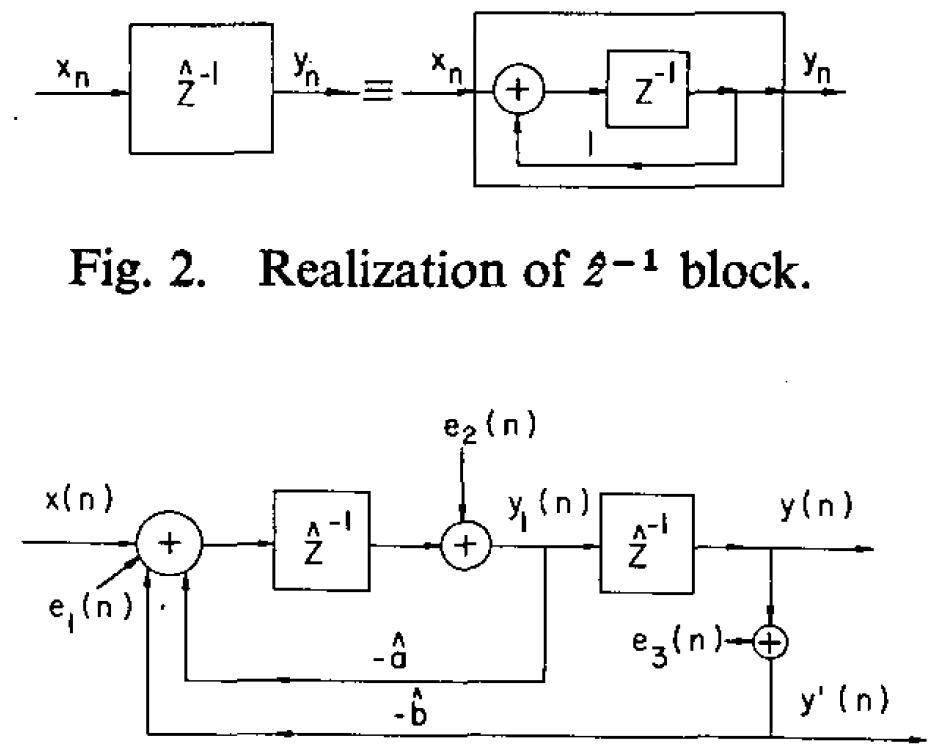
\includegraphics[width=0.4\textwidth]{Media/zHatRealization.PNG}
\caption{The realization of $ \hat{z} $ and the resultant filter}
\label{fig:zhatRealization}
\end{center}
\end{figure}.
\\
Unfortunately, we cant use this method as-is because implementing the recursive $ \hat{z} $ brings us back to our main issue of trying to implement a spatial recursive system.
\\
I am now facing a few options for advancing:
\begin{itemize}
\item{
\textbf{Finding a different solution in the spirit of the proposed one}
\\
Reading some papers that cited this paper, hoping to find a new idea which better suits our needs.
}
\item{
\textbf{Reevaluation of the problem}
\\
Check for an initially more robust IIR filter designs which will free us from the need of filter immunizing.
}
\end{itemize}
\section{2017 Dec 11$^{th}$}
\textbf{A research progress update mail} 

\begin{mdframed}
Prof. Cohen and Dr. Dvorkind 
Good afternoon. 
Since the presentation before Prof. Cohen's student group there has been some progress which I want to share.

brief reminder:

Were presented a spatial feedback based array architecture that enabled an IIR spatial response without any temporal processing.

Designing the result transfer function depends on knowing the range of the speaker. 

Our open issue was that when trying to implement a conventional IIR design (e.g. chevichev II) to the system's coefficients, the sensitivity to partial knowledge of the speaker's distance is unreasonable (i.e. in acoustic environment, we need to know its range with precision of around 1mm).

Research progress:

Since then, I tried to find an algorithm for "immunizing" the filter design for lower sensitivity to errors.

Dr. Dvorkind suggested that lower sensitivity to coefficient quantization errors may be equivalent to lower sensitivity to input errors (i.e. partial knowledge of the physical parameters such as range) when realizing the filter with high precision coefficients.

I then started to read papers that dealt with filter sensitivity issues and after few papers that were not very relevant (found it after reading them), I came across a very interesting paper from 1975.
[1]"New recursive digital filter structures having very low sensitivity and roundoff noise"
that dealt with the exact sensitivity issue that we experienced (i.e. poles that are to close to z=1 in z domain).
It suggested processing the signal around z=1 instead of z=0 (shifting the origin of z), resulting in a mere change of the coefficients and using integrators instead of a simple delay elements and only dealy with 2nd order IIR filters.

Another kind-of-related article was 
[2]"New first- and second-order very low sensitivity bandpass/bandstop complex digital filter sections"
that did not provide any new sensitivity reduction method but suggested that higher order IIR filters could be factored to 2nd order section (which is easily achieved by "tf2sos" Matlab function) and after immunizing each section one could re-synthesize the overall filter.

My current status:

After reading the mentioned paper, I tried to implement the method by:
Factoring the filter to 2nd order sections.
Implementing the suggested realization (from [1]) for each section.
Re-Synthesizing the overall filter with the immunized sections.
I found out that the immunizing method didn't actually change the transfer function (only adds two zeros for each section in z=0).
The change was only on the way of realizing the filter and when I re-synthesized the overall filter it was actually the same.
The conclusion is that the architecture must consist actual spatial integrators.  
 
The problem is that I didn't find a way to apply spatial integrators so currently I cant use the suggested method.

Current intended future tasks:

Now I am facing a few options for proceeding:
\begin{itemize}
\item{
\textbf{Finding a different solution in the spirit of the proposed one}
\\
Reading some papers that cited this paper, hoping to find a new idea which better suits our needs.
}
\item{
\textbf{Reevaluation of the problem}
\\
Check for an initially more robust IIR filter designs which will free us from the need of filter immunizing.
}
\end{itemize}

Should you have any suggestions, I will be glad to receive them.

Itay.
\end{mdframed}

\section{2017 Dec 23$^{rd}$}
In the past few weeks I tried to find filter design method that produce coefficients error robust transfer functions. The most interesting method (and also the most researched one) is the one originated in \cite{Agarwal1975NewNoise} \textbf{``New Recursive Digital Filter Structures Having Very Low Sensitivity and Roundoff Noise''} which was later called the ``delay-replacement'' and served as a fertile ground for the ``delta-operator'' which was thoroughly investigated in \cite{MiddletonRichardHandGoodwin1990DigitalSeries} \textbf{``Digital Control and Estimation: A Unified Approach (Prentice Hall Information and System Sciences Series)''}. Unfortunately, those methods basically meant that integrators should be used instead of simple delay components and clearly, in our proposed spatial feedback system a spatial integrator is not achievable.

\section{2017 Dec 30$^{th}$}
After failing to find a suitable method for low coefficients error sensitivity transfer functions, we decided to step back and re-model our problem. Our transfer function is 
$$
\ensuremath{
y_{\theta}^{\mathcal{F}}(\omega) 
=
\frac
{
\vecnot{\alpha}^{T}
\vecnot{d}_{\theta}
exp\left(-j\tau\right)
}
{
1
-
\vecnot{\beta}^{T}\vecnot{d}_{\theta}
exp\left(-j\tau\right)
}
x^{\mathcal{F}}(\omega)
}
$$
Practically, the error doesn't resemble a coefficients quantization noise which influences each coefficient separately. Here, the uncertainty translates to an unknown phase that equally influences all the coefficients but one. The denominator is $ 1 - \vecnot{\beta}^{T}\vecnot{d}_{\theta}e^{-j\omega (\tau_{pd}+\tau_{tx})} $, which obviously consists of one constant component (the $ 1 $) that cannot be diminished and the $ \vecnot{\beta}^{T}\vecnot{d}_{\theta}e^{-j\omega (\tau_{pd}+\tau_{tx})} $ which is this work's basic contribution. We modeled this in MATLAB using the four basic iir-design methods available:
\begin{itemize}
\item {butter}
\item {cheby1}
\item {cheby2}
\item {ellip}
\end{itemize}
and simulated increasing range estimation error to investigate its influence the transfer function's actual gain. We also checked multiple filter specifications.
\begin{figure}[!ht]
\begin{center}
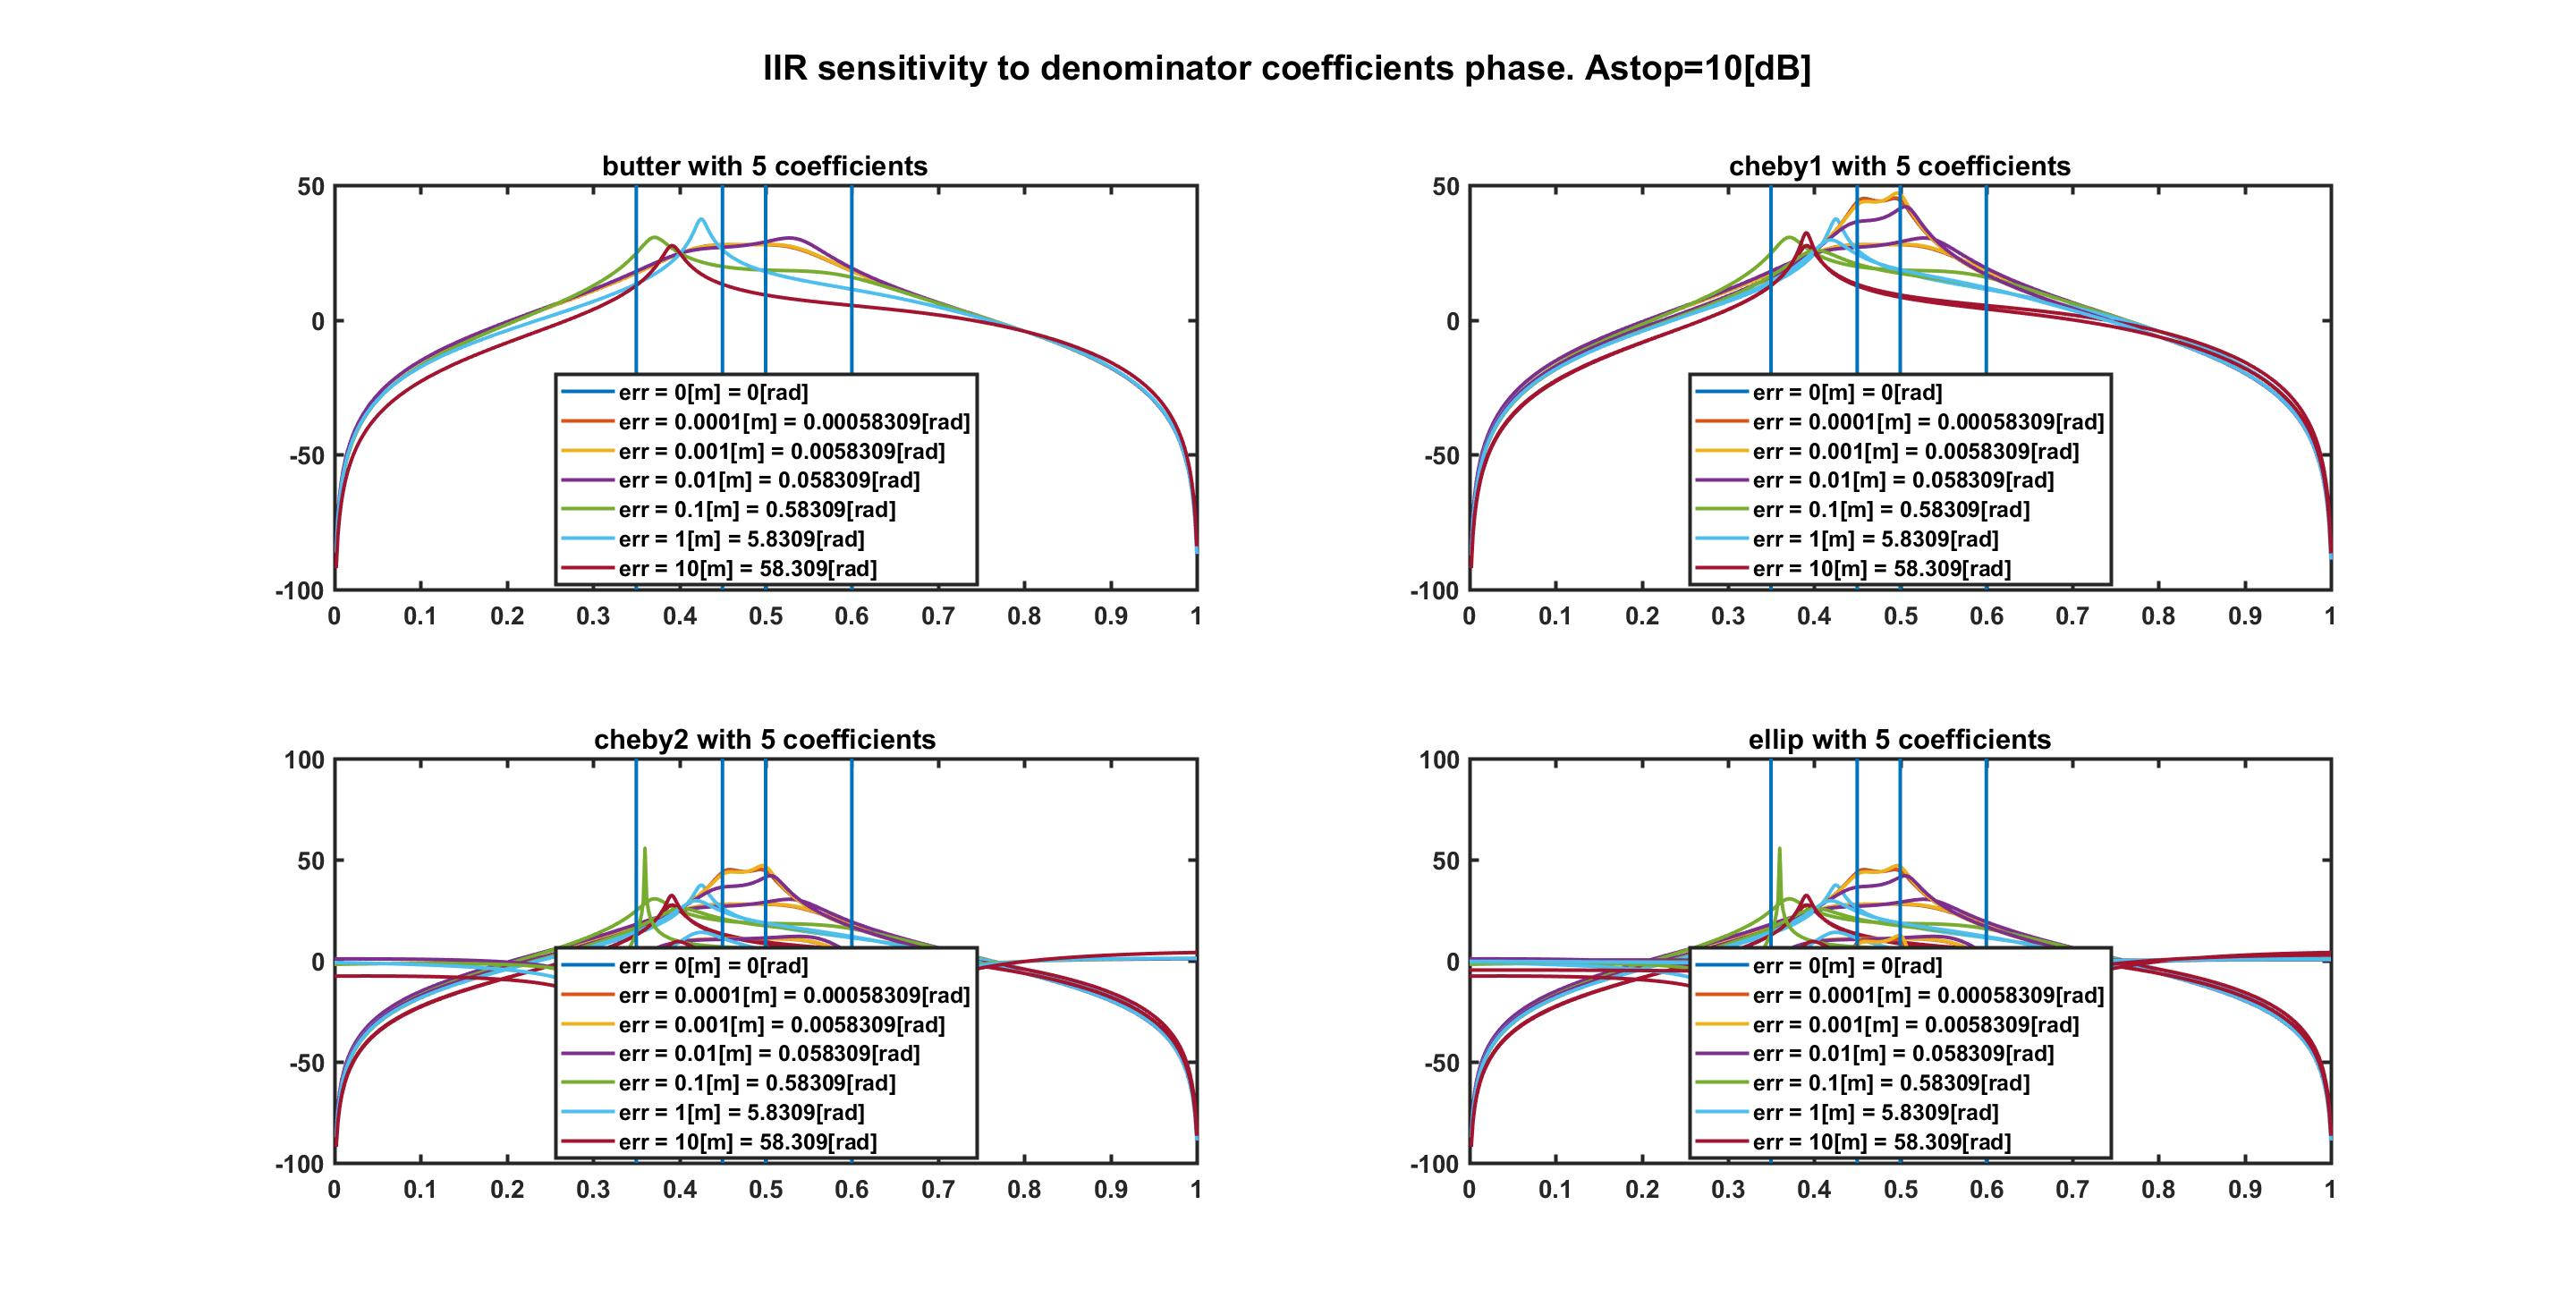
\includegraphics[width=1\textwidth]{Media/filterSensitivitySim/filtSensitivity10dB.jpg}
\end{center}
\end{figure}
\begin{figure}[!ht]
\begin{center}
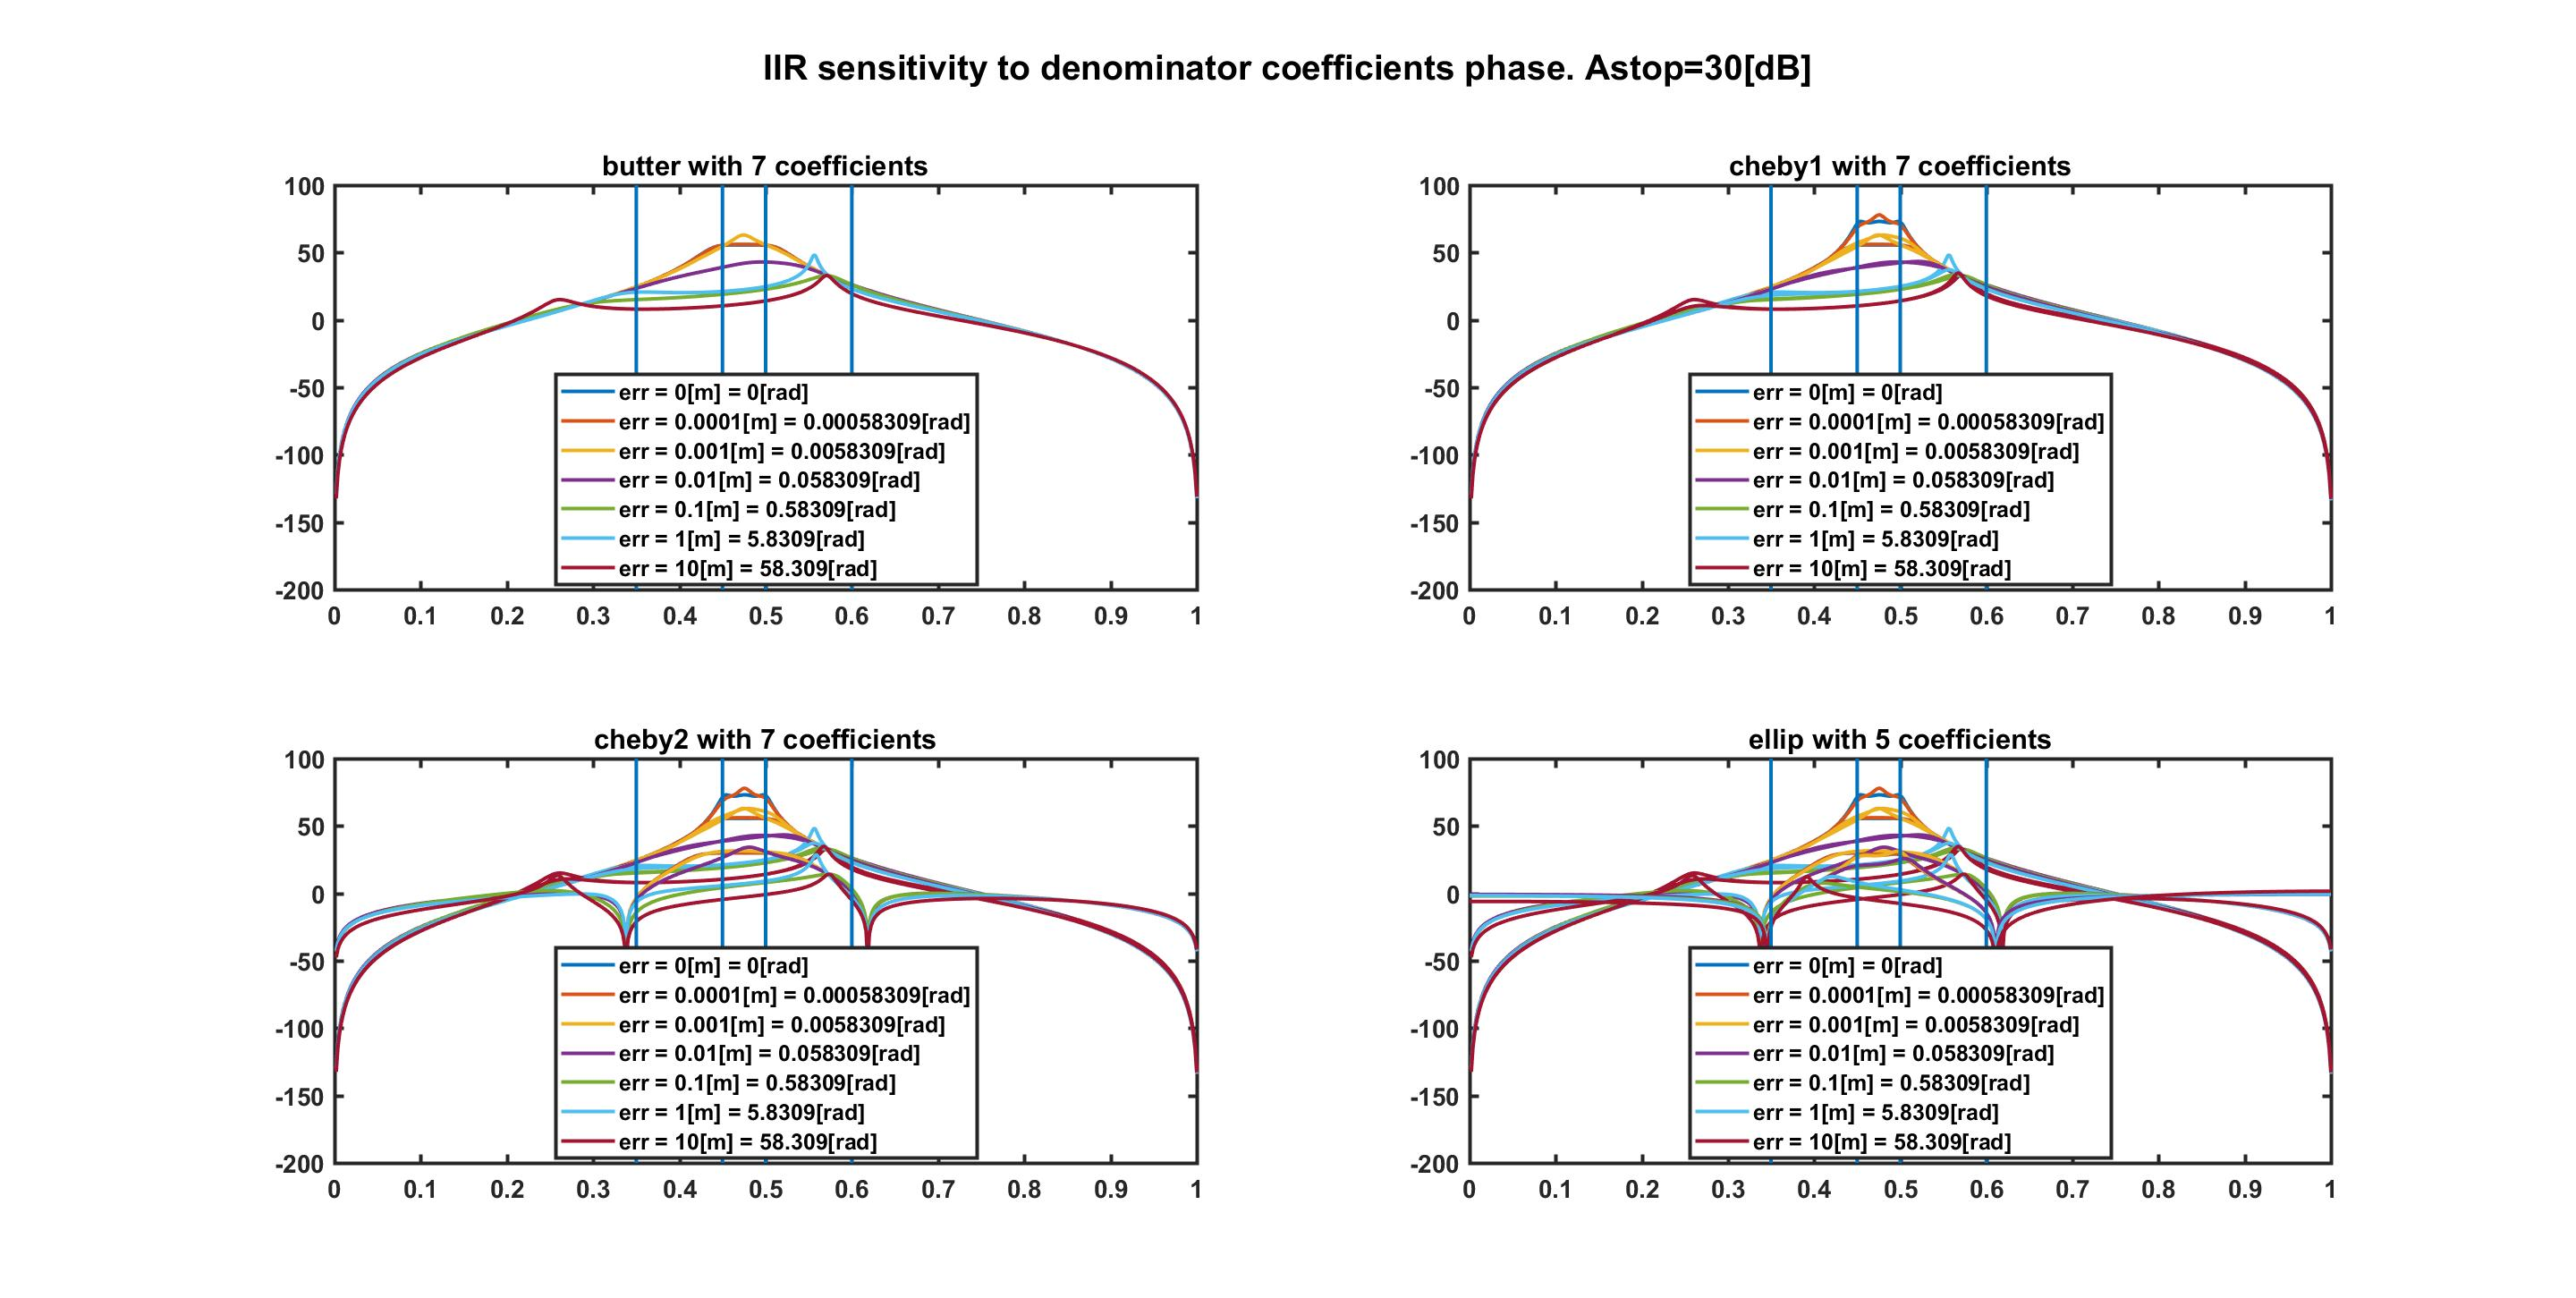
\includegraphics[width=1\textwidth]{Media/filterSensitivitySim/filtSensitivity30dB.jpg}
\end{center}
\end{figure}
\begin{figure}[!ht]
\begin{center}
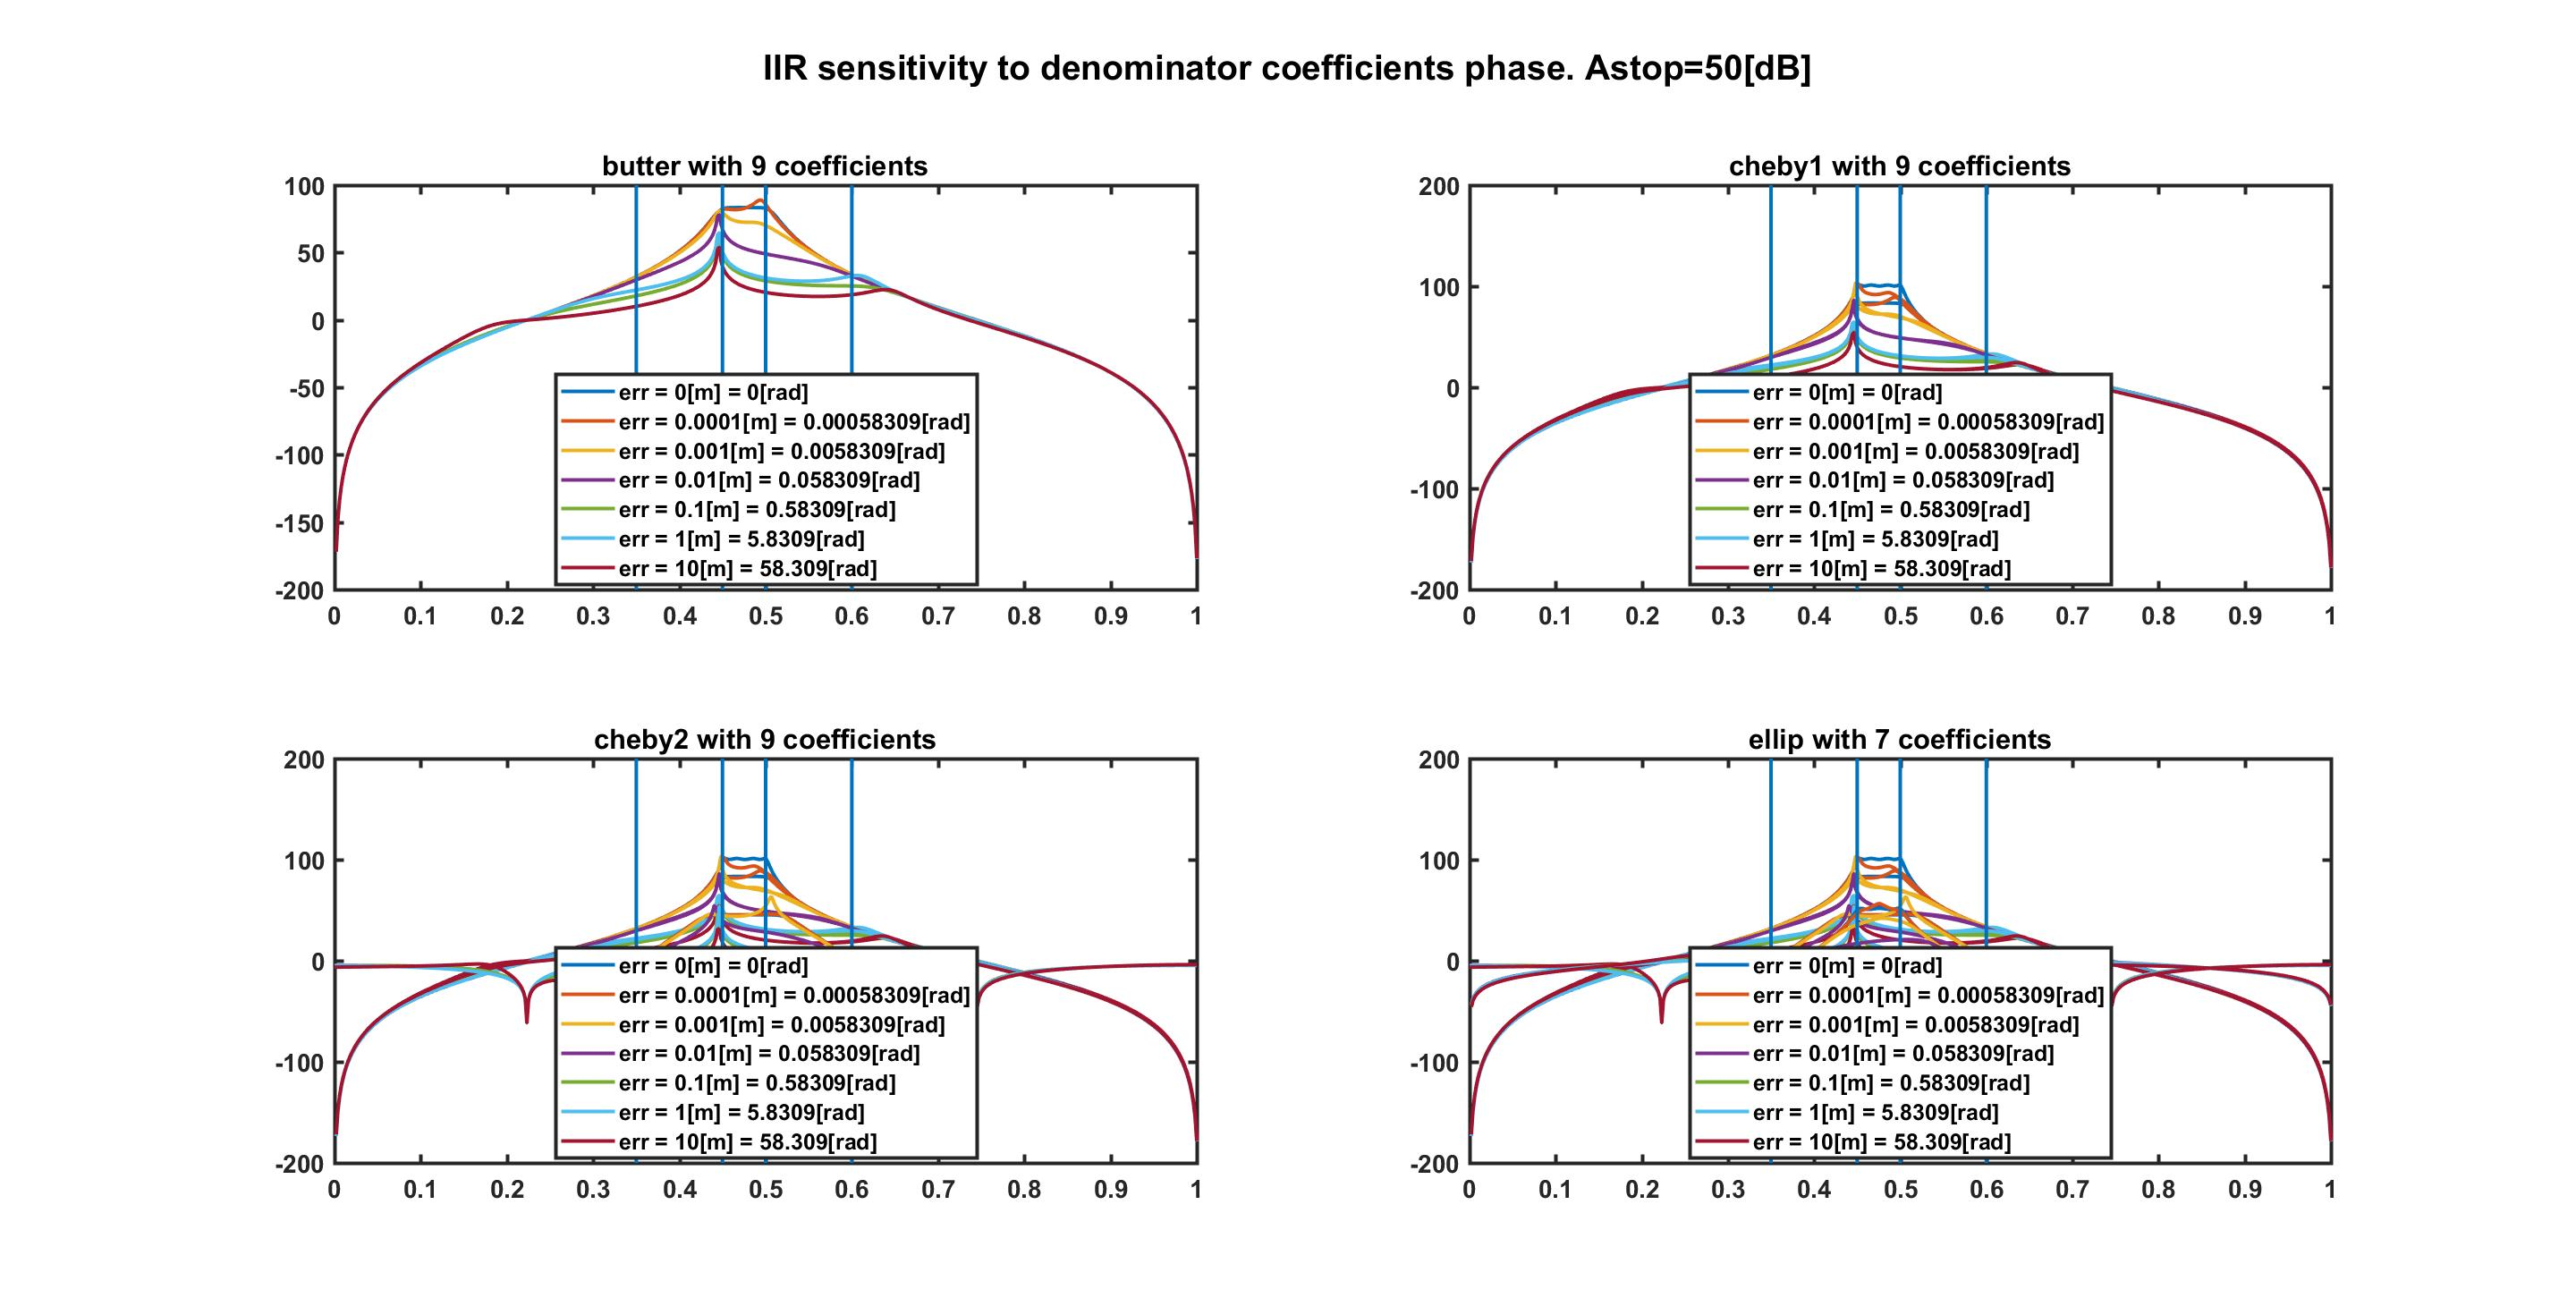
\includegraphics[width=1\textwidth]{Media/filterSensitivitySim/filtSensitivity50dB.jpg}
\end{center}
\end{figure}
\begin{figure}[!ht]
\begin{center}
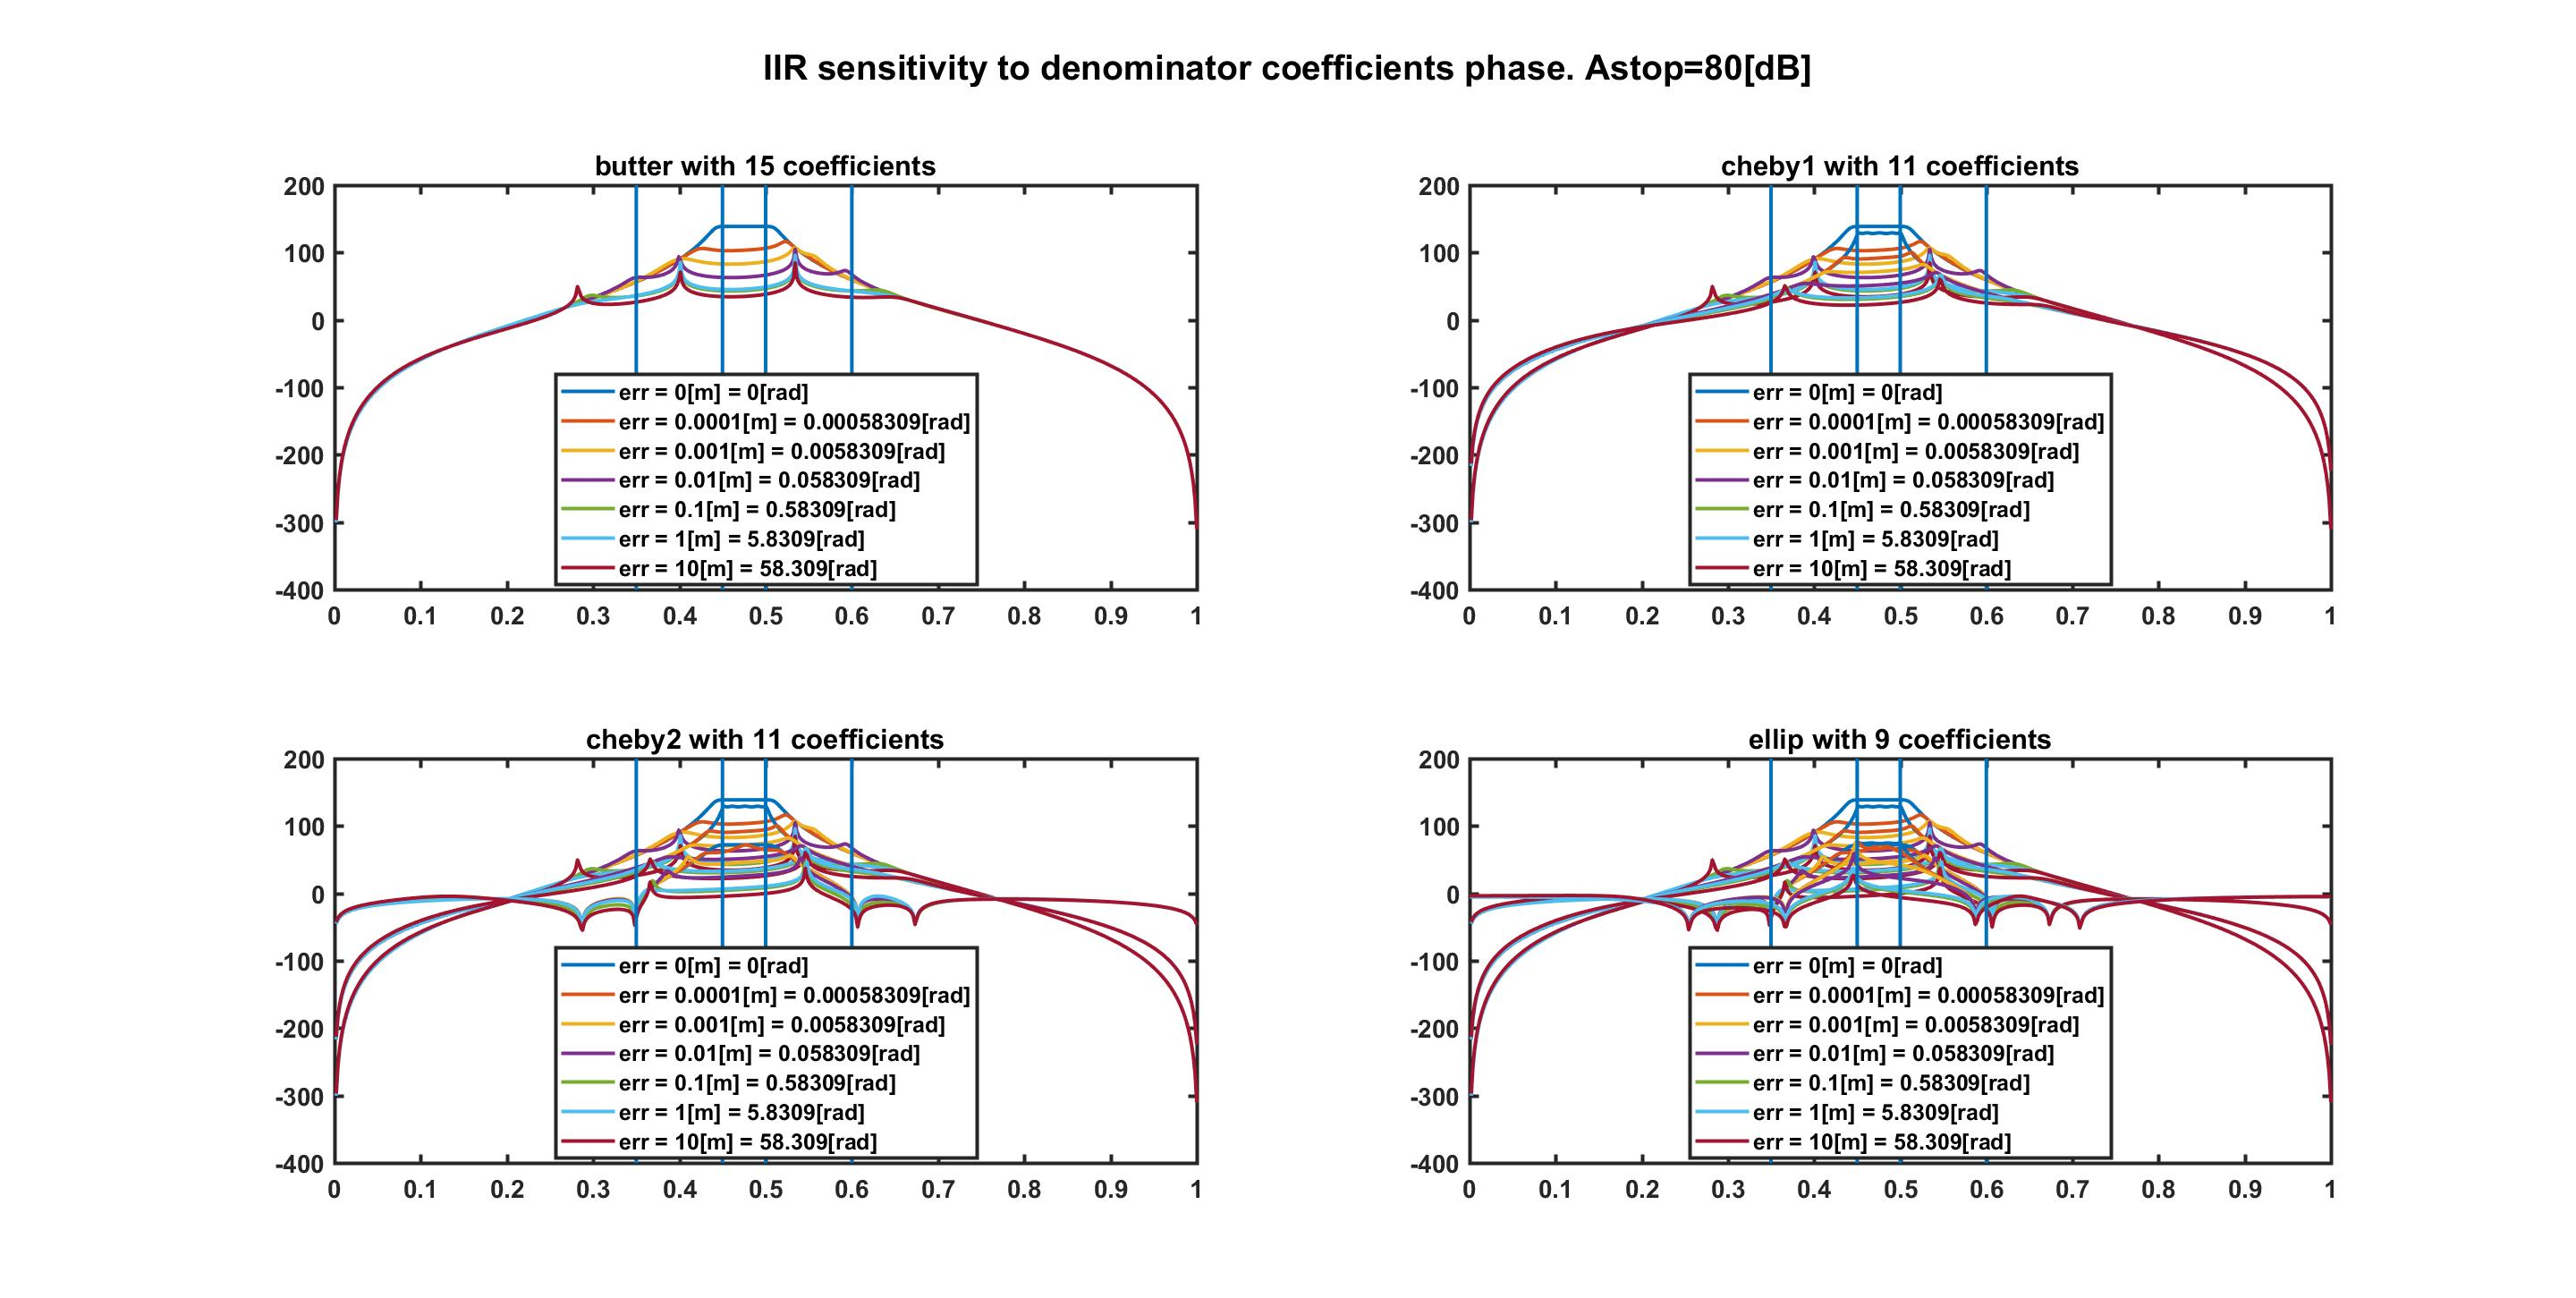
\includegraphics[width=1\textwidth]{Media/filterSensitivitySim/filtSensitivity80dB.jpg}
\end{center}
\end{figure}
\clearpage
\section{2017 Dec 31$^{st}$}
After discussing the results and the investigated methods, we decided to try some new approaches:
\begin{itemize}
\item {
\textbf{Solving a minimization problem}\\
We can formulate the next minimization problem 
\begin{equation*}
\begin{aligned}
& \underset{\vecnot{\alpha},\vecnot{\beta}}{\text{minimize}}
& & 
\left\lVert 
H_{d}(\theta) - H_{\vecnot{\alpha},\vecnot{\beta},\phi}(\theta)
\right\rVert^p
\\
& \text{subject to}
& & 0 < \phi \leq 2\pi, \; i = 1, \ldots, m.
\end{aligned}
\end{equation*}
where 
$ 
H_{\vecnot{\alpha},\vecnot{\beta},\phi}(\theta) =  
\frac
{
\vecnot{\alpha}^{T}
\vecnot{d}_{\theta}
}
{
1
-
\vecnot{\beta}^{T}\vecnot{d}_{\theta}
e^{-j\phi}
}
$
and 
$ 
H_{d}(\theta) =  
\frac
{
\vecnot{\alpha_{d}}^{T}
\vecnot{d}_{\theta}
}
{
\vecnot{\beta}_{d}^{T}\vecnot{d}_{\theta}
}
$
}. 
An easy was of modeling the problem is to use the polar ($\vecnot{r_{\vecnot{\alpha},\vecnot{\beta}}},\vecnot{\phi_{\vecnot{\alpha},\vecnot{\beta}}}$) representation of both zeros and poles (which still leaves $ 2N $ DOF) and coefficients.
\\
\textbf{Update (2018 Jan 14$^{th})$}
\\
An initial evaluation was made trying to solve the optimization problem 
\begin{equation*}
\begin{aligned}
& \underset{\vecnot{\alpha},\vecnot{\beta}}{\text{minimize}}
& & 
\left\lVert 
H_{d}(\theta) - H_{\vecnot{\alpha},\vecnot{\beta},\phi}(\theta)
\right\rVert^2
\\
& \text{subject to}
& & 0 < \phi \leq 2\pi, \; i = 1, \ldots, m.
\end{aligned}
\end{equation*}
by letting the radius $ r $ and azimuth $ \phi $ of both poles and zeros to be freely modified, thus enabling the filter to have complex coefficients. So far it didn't succeed and we are not sure that the problem is convex.
\\
Tsvi suggested modifying the optimization criterion to $ \left\lVert \right\rVert^\infty $ and maybe use a weighted version of the problem 
\begin{equation*}
\begin{aligned}
& \underset{\vecnot{\alpha},\vecnot{\beta}}{\text{minimize}}
& & 
\left\lVert 
\left(H_{d}(\theta) - H_{\vecnot{\alpha},\vecnot{\beta},\phi}(\theta)\right)^{T}\vecnot{w}
\right\rVert^\infty
\\
& \text{subject to}
& & 0 < \phi \leq 2\pi, \; i = 1, \ldots, m.
\end{aligned}
\end{equation*}
\item {
\textbf{Analog modulation of the feedback}
\\
Due to the high sensitivity of the system, we thought of analogically modulating the feedback such that in each modulation cycle, there will be a single sniping to the exact needed phase. 
\\
It should be mathematically investigated.
\\
\textbf{Update (2018 Jan 4$^{th})$}
\\
After brief mathematical development, the frequency domain dependency is
$$
\vecnot{x}^{\mathcal{F}}_{\theta}(\omega) = 
x^{\mathcal{F}}(\omega)
\vecnot{d}_{\theta}
e^{-j\omega\tau_{pd}}
+
\vecnot{d}_{\theta}
\vecnot{\beta}^{T}
e^{-j\omega(\tau_{pd}+\tau_{tx})}
\vecnot{x}_{\theta}^{\mathcal{F}}(\omega+\omega_{feedback})
$$
where $ \omega_{feedback} $ is the feedback modulation frequency so a linear transfer function can no longer be extracted from it. 
}
\item {
\textbf{Emitting a synthetic dual-close-harmony sync signal}
\\
The purpose of emitting dual harmonies with close frequencies is to receive a single low-frequency harmony which is centered on the difference between the two frequencies, thus improving the phase-dependent delay estimation.
\\
\textbf{Update (2018 Jan 14$^{th})$}
\\
This option is currently out main focus. we are now creating a matlab recursive simulation of two transponders scenario in which the system transmits a synthetic low frequency sync signal and also generates filtered feedback from the reflected signals, thus generating sot of all-pole system.
\\
For now, out prediction is that when the phase of the $ \vecnot{\beta} $ coefficients is set correctly, the received energy will be maximal and therefore we can use counter-gradient methods to dynamically ``lock'' the system on an object after steering the synthetic system poles to its direction.
\\
We want to evaluate the affects of both update rate and phase step size on the system's performance.
}
\item {
\textbf{Internal feedback architecture}
\\
I presented to Tsvi an idea of internal feedback architecture that uses the input's phases to phase modulate the feedback signal without the transmission and propagation delay.
\\
For now we ignore this option because Tsvi feels that it actually returns to the spatio-temporal processing papers that are not achieving the concept of spatial-only filtering and he also claims that inherently, we actually perform some kind of DOA estimation.
\\
\textbf{Update (2018 Jan 14$^{th})$}
\\
After math examination, the feedback phases hold not only the spatial information. They are also influenced by the source signal's amplitude. Therefore, in the multiple sources scenario this method suffers the same problem of doa-estimation necessity.
\begin{figure}[!h]
\begin{center}
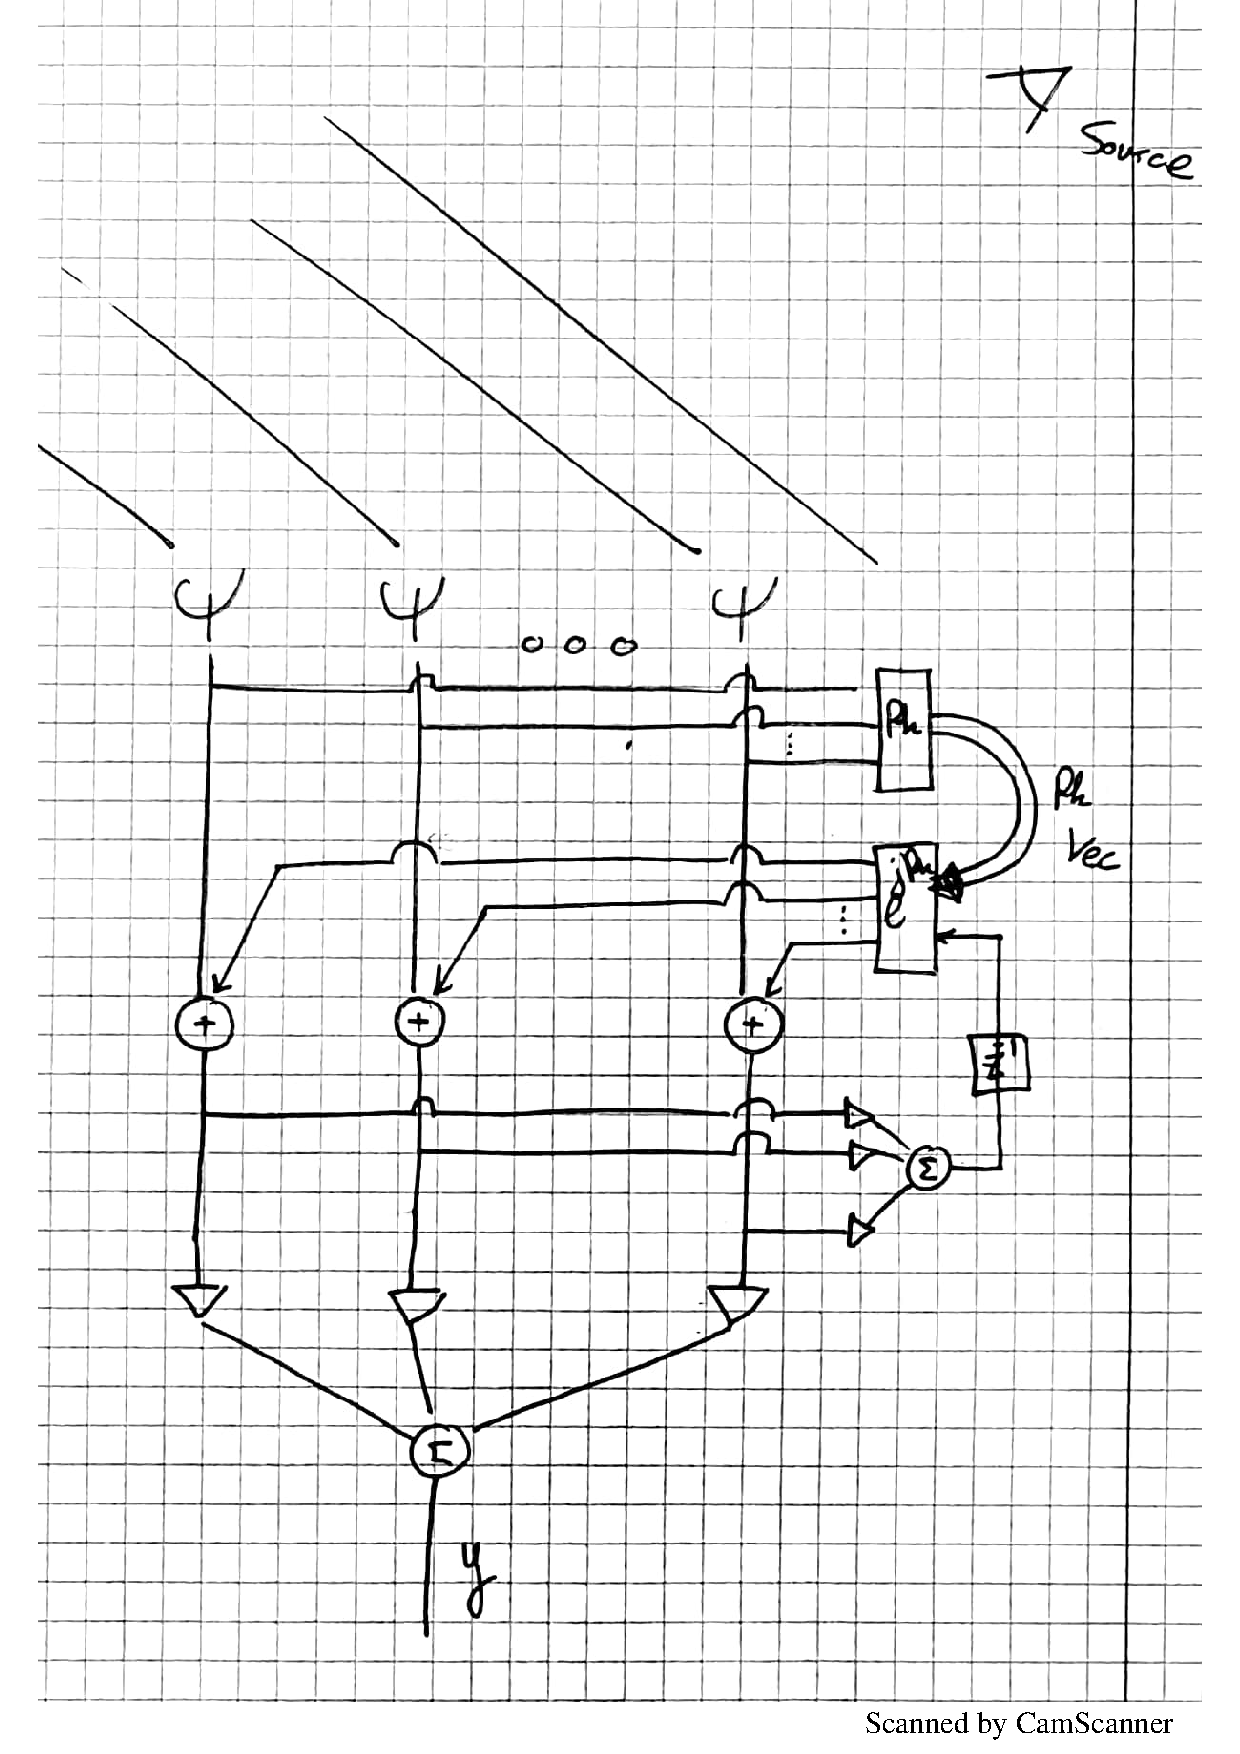
\includegraphics[width=0.7\textwidth]{Media/local_feedback_arch.pdf}
\caption{The suggested Internal feedback architecture}
\end{center}
\end{figure}.
}
\end{itemize}

\section{2018 Feb 20th$^{th}$}
After presenting the latest progress to Prof. Cohen and his students, some comments were made:
\begin{itemize}
\item{
Add an ideal-case simulation to prove that an IIR like spatial response is actually achievable.
}
\item{
Add a symbolic signal flow to help the reader understand the feedback.
}
\item{
Try to simulate a single sensor simulation.
\\
NOTE: I personally think that the minimal number of sensor is 2 to achieve a spatial sampler.
}
\item{
Try and find citing papers of Wen and show that no similar work to our research was made until now.
}
\item{
Add an intuitive paragraph that should convince the reader that a spatial IIR is achievable.
}
\item{
Consider re-focusing the research to a single stationary source of CW signal in a flat channel environment.
}
\end{itemize}
After the presentation I read ``Cram{\'{e}}r-Rao bounds for estimating range, velocity, and direction with a sensor array'' \cite{Dogandzic2000Cramer-RaoArray} and Tsvi suggested that I should try and apply their methods of finding the CRLB to our signal model which involves the feedbacks. so now this is my main focus.

\section{Simulations}
A comprehensive simulation was created for both the demonstration of ``spatial-IIR'' system response and the study of its controllability/limitations.
\subsection{Simulation structure \& parameters}
\subsubsection{simulation scenario}
In each simulation one can set multiple parameters:
\begin{itemize}
\item{
Array structure and azimuth.
}
\item{
Object's location as a time-dependent function.
}
\item{
Signals characteristics such as sync-signal frequency and duration.
}
\end{itemize}
\subsubsection{simulation structure}
For an accurate simulation of the physical environment the simulation should support an active (i.e. transmitting) array and responsive (i.e. reflective) objects. The nominal scenario consists of a array that emits a sync signal while the object reflects it back to the array. In addition to its own emitted sync signal, the array can also emit a feedback signal, synthesized from the received object-reflected signal which imping each sensor. 
\begin{itemize}
\item{
The simulation engine pre-computes the minimal distance between the object and the array throughout the entire simulated period.
}
\item{
According to the minimal distance and the propagation velocity of the signal, a simulation segment duration is set to ensure that all samples in the segment can be calculated from the pre-segment history, hence no dependencies exist between samples a particular segment.
}
\end{itemize}
\clearpage
\small
{
\bibliographystyle{unsrt}
\bibliography{./Modules/Mendeley,./Modules/LocalBib}
}
\end{document}